
%  Multigrid FSP for the RDME — v6 (streamlined)
%  Aditya Dendukuri

\documentclass[10pt,aspectratio=169]{beamer}

\usetheme{Boadilla}
\usecolortheme{seahorse}
\setbeamertemplate{navigation symbols}{}
\setbeamerfont{frametitle}{size=\normalsize,series=\bfseries}
\setbeamerfont{title}{size=\large,series=\bfseries}
\setbeamertemplate{bibliography item}[text]

\usepackage{amsmath,amssymb,bm,mathtools}
\usepackage{tikz}
\usetikzlibrary{arrows.meta,positioning,patterns,decorations.pathreplacing,calc}
\usepackage{graphicx}
\usepackage{booktabs}
\usepackage{xcolor}
\usepackage{colortbl}
\usepackage{pifont}

\graphicspath{{figures/}}

\newcommand{\Bin}{\operatorname{Bin}}
\newcommand{\calR}{\mathcal{R}}
\newcommand{\calP}{\mathcal{P}}

\definecolor{fastblue}{RGB}{31,119,180}
\definecolor{slowred}{RGB}{214,39,40}
\definecolor{coarsegreen}{RGB}{44,160,44}
\definecolor{intercolor}{RGB}{255,140,0}
\definecolor{myblue}{RGB}{31,119,180}
\definecolor{mygray}{RGB}{80,80,80}
\definecolor{activegreen}{RGB}{44,160,44}
\definecolor{equilpurple}{RGB}{148,103,189}

\title[Multigrid FSP for RDME]{%
  Multigrid Finite State Projection\\
  for the Reaction-Diffusion Master Equation}
\author{Aditya Dendukuri}
\institute[UCSB]{University of California, Santa Barbara}
\date{}

\begin{document}

\begin{frame}\titlepage\end{frame}


% ================================================================
%  1. CME
% ================================================================
\begin{frame}{The Chemical Master Equation}

  \begin{columns}[T]
    \begin{column}{0.50\textwidth}
      Integer counts $n \in \mathbb{Z}_{\geq 0}$ evolving by stochastic reactions.
      The probability distribution $p(n,t)$ satisfies:
      \[
        \dot{p} = A\,p
      \]

      \begin{alertblock}{SSA vs.\ CME}
        \textbf{SSA} samples individual trajectories.\\[0.3em]
        \textbf{CME} gives the \emph{exact} joint distribution
        $p(n,t)$ --- rare events, tails, bimodal structure, no ensemble noise.
      \end{alertblock}

      \medskip
      {\small
        \textbf{FSP}: truncate $A$ to a finite support $\mathcal{S}$,
        solve $\dot p = Ap$ via $\mathrm{expv}$.
        Expand $\mathcal{S}$ at the boundary; prune negligible states.
      }
    \end{column}
    \begin{column}{0.46\textwidth}
      \textbf{Birth-death: $\emptyset \xrightarrow{\lambda} X \xrightarrow{\mu n} \emptyset$}
      \begin{center}
      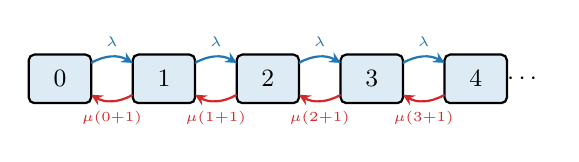
\begin{tikzpicture}[scale=0.88,every node/.style={font=\small},>=stealth]
        \foreach \n in {0,1,2,3,4}{
          \draw[thick,fill=myblue!15,rounded corners=2pt]
            (\n*1.5,0) rectangle (\n*1.5+0.9,0.7);
          \node at (\n*1.5+0.45,0.35) {$\n$};
        }
        \node at (4*1.5+1.15,0.35) {$\cdots$};
        \foreach \n in {0,1,2,3}{
          \draw[->,fastblue,thick,bend left=30]
            (\n*1.5+0.9,0.58) to node[above,font=\tiny]{$\lambda$}
            ({(\n+1)*1.5},0.58);
          \draw[->,slowred,thick,bend left=30]
            ({(\n+1)*1.5},0.12) to node[below,font=\tiny]{$\mu(\n{+}1)$}
            (\n*1.5+0.9,0.12);
        }
      \end{tikzpicture}
      \end{center}
      \vspace{0.3em}
      Stationary: $\mathrm{Pois}(\lambda/\mu)$.
      \vspace{0.4em}
      \begin{center}
      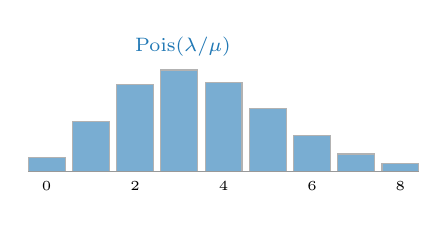
\begin{tikzpicture}[scale=0.78]
        \foreach \n/\h in {0/0.13,1/0.45,2/0.79,3/0.92,4/0.81,5/0.57,6/0.33,7/0.16,8/0.07}{
          \fill[myblue!60] (\n*0.72,0) rectangle (\n*0.72+0.60,\h*1.8);
          \draw[black!30] (\n*0.72,0) rectangle (\n*0.72+0.60,\h*1.8);
        }
        \draw[black!40] (0,0)--(8*0.72+0.60,0);
        \foreach \n in {0,2,4,6,8}{\node[below,font=\tiny] at (\n*0.72+0.30,0) {\n};}
        \node[above,font=\scriptsize,myblue] at (3.5*0.72,1.72) {$\mathrm{Pois}(\lambda/\mu)$};
      \end{tikzpicture}
      \end{center}
    \end{column}
  \end{columns}

\end{frame}


% ================================================================
%  2. RDME
% ================================================================
\begin{frame}{The RDME: exact but exponentially large}

  \begin{columns}[T]
    \begin{column}{0.50\textwidth}
      Divide the domain into $K{\times}K$ voxels.
      Each voxel $\mathbf{k}$ holds count $n_\mathbf{k}$.

      \medskip
      Two event types:
      \begin{itemize}\setlength\itemsep{0.35em}
        \item \textcolor{slowred}{\textbf{Reactions}} inside $\mathbf{k}$:
              propensity $\alpha(n_\mathbf{k})$
        \item \textcolor{fastblue}{\textbf{Diffusion}} $\mathbf{k}\leftrightarrow\mathbf{l}$:
              rate $d{=}D/h^2$, one molecule
      \end{itemize}

      \medskip
      Joint distribution $p(\{n_\mathbf{k}\},t)$ satisfies $\dot p = Ap$ \textbf{(RDME)}.

      \begin{alertblock}{The curse of dimensionality}
        State space: $n_{\max}^{K^2}$.\\
        A $200{\times}200$ grid is \textbf{completely intractable} directly.\\[0.3em]
        \textbf{Key locality:} diffusion only couples \emph{adjacent} voxels
        --- this structure enables a principled decomposition.
      \end{alertblock}
    \end{column}
    \begin{column}{0.46\textwidth}
      \begin{center}
      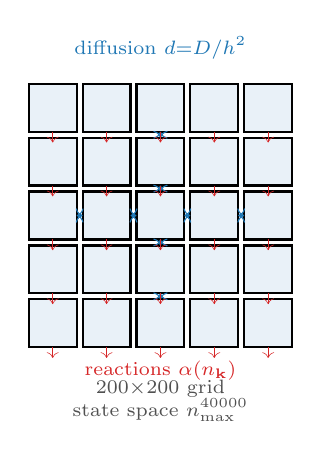
\begin{tikzpicture}[scale=0.76,every node/.style={font=\scriptsize}]
        \foreach \i in {0,...,4}\foreach \j in {0,...,4}{
          \draw[thick,fill=myblue!10](\i*0.9,\j*0.9)rectangle(\i*0.9+0.8,\j*0.9+0.8);
        }
        \foreach \i in {0,...,3}{
          \draw[<->,fastblue,thin](\i*0.9+0.8,2*0.9+0.4)--(\i*0.9+0.9,2*0.9+0.4);
        }
        \foreach \j in {0,...,3}{
          \draw[<->,fastblue,thin](2*0.9+0.4,\j*0.9+0.8)--(2*0.9+0.4,\j*0.9+0.9);
        }
        \foreach \i in {0,...,4}\foreach \j in {0,...,4}{
          \draw[->,slowred,very thin](\i*0.9+0.4,\j*0.9+0.0)--(\i*0.9+0.4,\j*0.9-0.18);
        }
        \node[fastblue] at (2.2,5.0){diffusion $d{=}D/h^2$};
        \node[slowred]  at (2.2,-0.4){reactions $\alpha(n_\mathbf{k})$};
        \node[mygray,align=center] at (2.2,-0.9){$200{\times}200$ grid\\state space $n_{\max}^{40000}$};
      \end{tikzpicture}
      \end{center}
    \end{column}
  \end{columns}

\end{frame}


% ================================================================
%  3. Three voxel regimes
% ================================================================
\begin{frame}{Three voxel regimes: adaptive classification at each step}

\begin{columns}[T]
\column{0.50\textwidth}

Every voxel $\mathbf{k}$ belongs to one of three regimes, reassigned each step:

\medskip
\begin{block}{\textcolor{activegreen!80!black}{Active} (wavefront)}
  Full CME distribution $p_k(n)$ tracked.\\
  Evolved by the multigrid V-cycle --- captures joint dynamics of neighbouring voxels.\\
  \emph{Typically a thin ring around the wavefront.}
\end{block}

\begin{block}{\textcolor{equilpurple}{Equilibrated} (interior/exterior)}
  Full distribution $p_k(n)$ tracked.\\
  Evolved cheaply by a \textbf{Galerkin-reduced single-voxel CME}:
  \[
    Q_k^{\rm eff}[n{\to}n{+}1] = r_b + d\sum_{\ell\sim k}\mu_\ell
  \]
  Uses neighbour means $\mu_\ell = \langle n_\ell\rangle$ as effective rates.\\
  Near-stationary $\Rightarrow$ small Krylov dim.
\end{block}

\begin{block}{\textcolor{mygray}{Empty}}
  Not tracked ($P(n{=}0)=1$).\\
  Activated \emph{organically}: $P(n_\ell{>}0)>\varepsilon$ in any neighbour.
\end{block}

\column{0.46\textwidth}
\vspace{0.2em}
\begin{center}
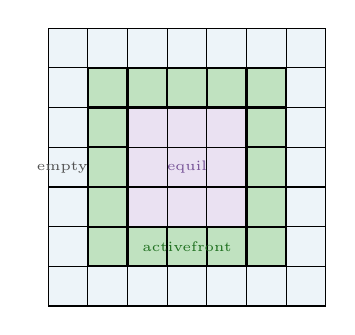
\begin{tikzpicture}[scale=0.70,every node/.style={font=\scriptsize}]
  \def\vs{0.72}
  % Empty exterior
  \foreach \i in {0,...,6}\foreach \j in {0,...,6}{
    \draw[fill=myblue!8](\i*\vs,\j*\vs)rectangle(\i*\vs+\vs,\j*\vs+\vs);
  }
  % Equil interior
  \foreach \i in {2,...,4}\foreach \j in {2,...,4}{
    \draw[fill=equilpurple!20](\i*\vs,\j*\vs)rectangle(\i*\vs+\vs,\j*\vs+\vs);
  }
  % Active ring
  \foreach \xk/\yk in {1/1,2/1,3/1,4/1,5/1,1/5,2/5,3/5,4/5,5/5,1/2,1/3,1/4,5/2,5/3,5/4}{
    \draw[fill=activegreen!30,thick](\xk*\vs,\yk*\vs)rectangle(\xk*\vs+\vs,\yk*\vs+\vs);
  }
  \node[mygray,font=\tiny] at (0.36*\vs,3.5*\vs){empty};
  \node[equilpurple!80!black,font=\tiny,align=center] at (3.5*\vs,3.5*\vs){equil};
  \node[activegreen!70!black,font=\tiny,align=center] at (3.5*\vs,1.5*\vs){active\newline front};
\end{tikzpicture}
\end{center}

\medskip
{\footnotesize
  \textbf{Key:} equil voxels track the \emph{full} distribution (not just the mean),
  so cross-basin events and non-Poisson tails are preserved.\\[0.4em]
  The multigrid V-cycle (next slide) handles \emph{only} the thin active front ---
  where inter-voxel correlations matter most.
}
\end{columns}

\end{frame}


% ================================================================
%  4. True spatial multigrid
% ================================================================
\begin{frame}{Spatial multigrid V-cycle: three levels, one time step}

\begin{columns}[T]
\column{0.48\textwidth}

\textbf{Hierarchy over active voxels:}
\begin{itemize}\setlength\itemsep{0.25em}
  \item \textbf{L0} individual voxels: $p_k(n)$, $w$ states
  \item \textbf{L1} adjacent pairs: $p(N_2{=}n_1{+}n_2)$, 1-D
  \item \textbf{L2} $2{\times}2$ quads: $p(N_4)$, 1-D \quad[coarsest]
\end{itemize}

\medskip
\textbf{One V-cycle = exactly $\Delta t$:}\\[0.3em]
{\small $\alpha_{\rm pre}\Delta t$ \;+\; $(1{-}2\alpha)\Delta t$ \;+\; $\alpha_{\rm post}\Delta t \;=\; \Delta t$}

\medskip
\begin{enumerate}\setlength\itemsep{0.22em}
  \item \textbf{Pre-smooth} L0: per-voxel expv \;[$\alpha_{\rm pre}\Delta t$]
  \item \textbf{Restrict} L0$\to$L1: $p_{12}(N_2) = p_1 * p_2$
  \item \textbf{Restrict} L1$\to$L2: $p_{1234}(N_4) = p_{12} * p_{34}$
  \item \textbf{Coarse solve} L2: 1-D CME \;[$(1{-}2\alpha)\Delta t$]
  \item \textbf{Correct} L2$\to$L1: $p_{12}^{\rm new} \propto p_{12}\times E[C(N_4)\!\mid\!N_2]$
  \item \textbf{Correct} L1$\to$L0: $p_k^{\rm new} \propto p_k\times E[C(N_2)\!\mid\!n_k]$
  \item \textbf{Post-smooth} L0: per-voxel expv \;[$\alpha_{\rm post}\Delta t$]
\end{enumerate}

\medskip
{\small \textbf{Multiplicative correction at each level:}
\[
  p_k^{\rm new}(n) \propto p_k(n)\!\sum_N \frac{p^{\rm new}[N]}{p^{\rm old}[N]}\,p_{\rm other}(N{-}n)
\]
Exact for existing $N$; identity fallback for new $N$.
}

\column{0.49\textwidth}
\begin{center}
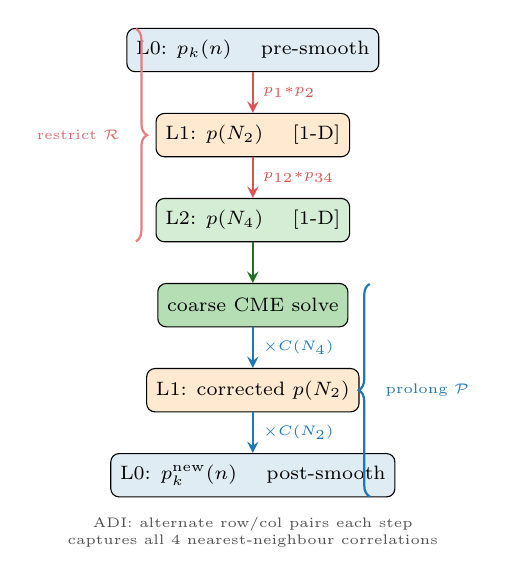
\begin{tikzpicture}[>=stealth,scale=0.90,every node/.style={font=\small}]

  % ── left: V-cycle diagram ────────────────────────────────────────
  \def\bw{3.0}
  \def\bh{0.55}

  % L0
  \node[draw,rounded corners=3pt,fill=myblue!14,minimum width=\bw cm,
        minimum height=\bh cm,align=center,font=\scriptsize] (L0pre) at (0,3.3)
    {L0: $p_k(n)$ \quad pre-smooth};

  % L1
  \node[draw,rounded corners=3pt,fill=intercolor!18,minimum width=2.4cm,
        minimum height=\bh cm,align=center,font=\scriptsize] (L1) at (0,2.1)
    {L1: $p(N_2)$ \quad [1-D]};

  % L2 / coarse solve
  \node[draw,rounded corners=3pt,fill=coarsegreen!20,minimum width=1.8cm,
        minimum height=\bh cm,align=center,font=\scriptsize] (L2) at (0,0.9)
    {L2: $p(N_4)$ \quad [1-D]};

  \node[draw,rounded corners=3pt,fill=coarsegreen!35,minimum width=1.8cm,
        minimum height=\bh cm,align=center,font=\scriptsize] (L2s) at (0,-0.3)
    {coarse CME solve};

  % L1 corrected
  \node[draw,rounded corners=3pt,fill=intercolor!18,minimum width=2.4cm,
        minimum height=\bh cm,align=center,font=\scriptsize] (L1c) at (0,-1.5)
    {L1: corrected $p(N_2)$};

  % L0 corrected
  \node[draw,rounded corners=3pt,fill=myblue!14,minimum width=\bw cm,
        minimum height=\bh cm,align=center,font=\scriptsize] (L0post) at (0,-2.7)
    {L0: $p_k^{\rm new}(n)$ \quad post-smooth};

  % Restriction arrows
  \draw[->,thick,slowred!80] (L0pre)--(L1)
    node[midway,right,slowred!80,font=\tiny]{$p_1{*}p_2$};
  \draw[->,thick,slowred!80] (L1)--(L2)
    node[midway,right,slowred!80,font=\tiny]{$p_{12}{*}p_{34}$};
  \draw[->,thick,coarsegreen!70!black] (L2)--(L2s);

  % Prolongation arrows
  \draw[->,thick,fastblue] (L2s)--(L1c)
    node[midway,right,fastblue,font=\tiny]{$\times C(N_4)$};
  \draw[->,thick,fastblue] (L1c)--(L0post)
    node[midway,right,fastblue,font=\tiny]{$\times C(N_2)$};

  % Brace labels
  \draw[decorate,decoration={brace,amplitude=4pt},thick,slowred!60]
    (-1.65,3.6)--(-1.65,0.6)
    node[midway,left,slowred!70,font=\tiny,xshift=-2pt]{restrict $\calR$};
  \draw[decorate,decoration={brace,amplitude=4pt,mirror},thick,fastblue]
    (1.65,-0.0)--(1.65,-3.0)
    node[midway,right,fastblue,font=\tiny,xshift=2pt]{prolong $\calP$};

  % ADI note
  \node[mygray,font=\tiny,align=center] at (0,-3.5)
    {ADI: alternate row/col pairs each step\\captures all 4 nearest-neighbour correlations};

\end{tikzpicture}
\end{center}
\end{columns}

\end{frame}


% ================================================================
%  5. BD 200x200 result
% ================================================================
\begin{frame}{Result: A$\to$2A wavefront on a $200{\times}200$ RDME}
\begin{center}
  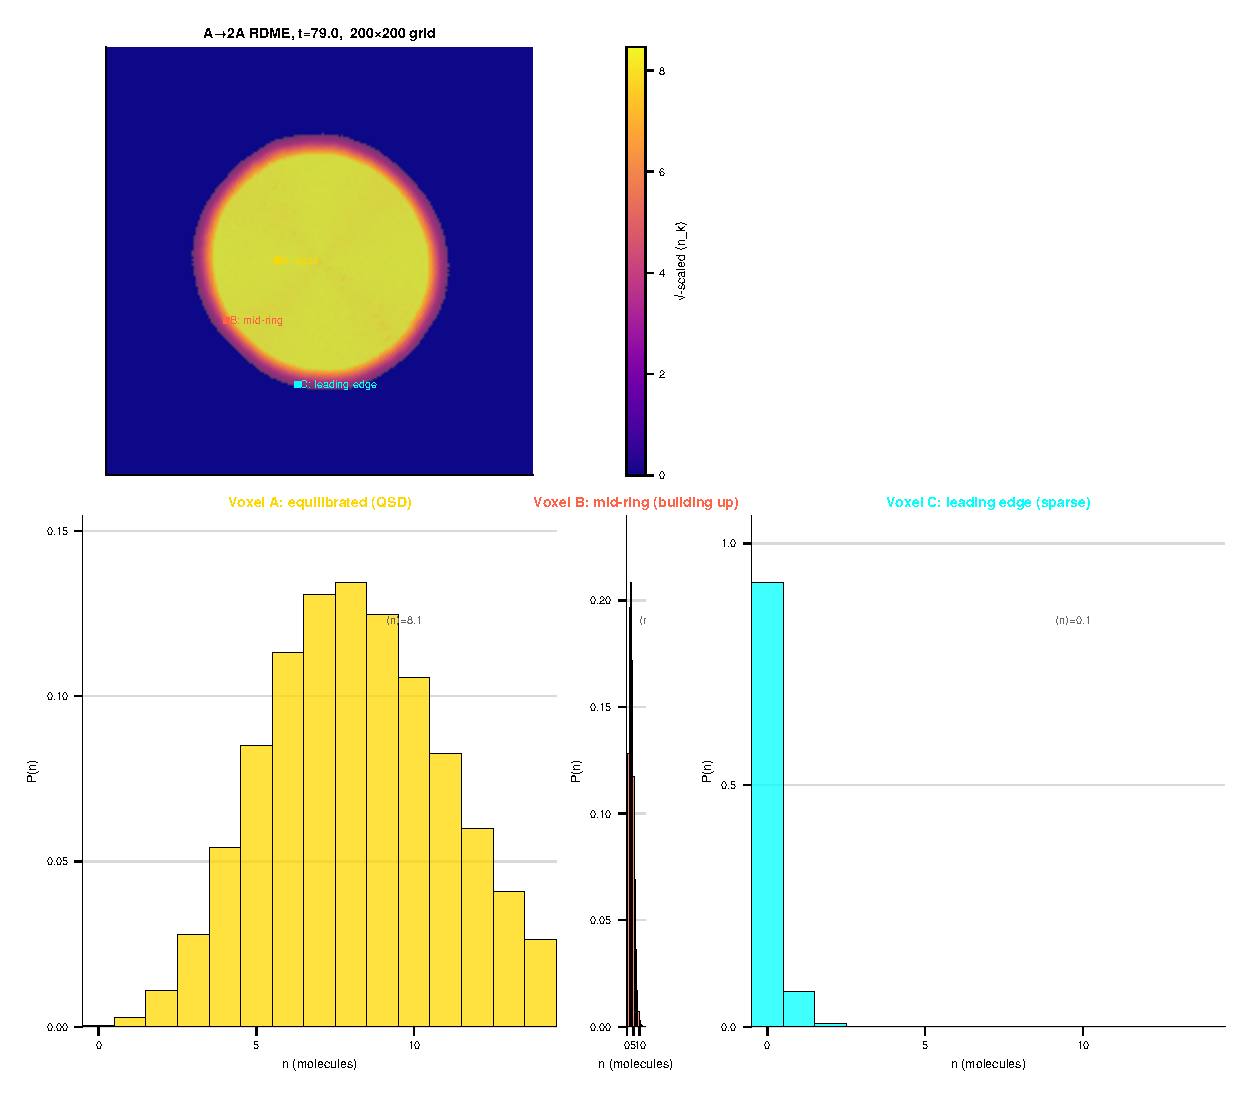
\includegraphics[width=0.90\textwidth,keepaspectratio]{fig_wave_snapshot}
\end{center}
\vspace{-0.4em}
{\footnotesize
  Branching-death RDME ($k_b{=}0.5$, $k_d{=}0.1$, $D{=}1.0$), $200{\times}200$ grid.
  IC: disc of radius 4 voxels at centre.
  \textbf{Top}: $\sqrt{\langle n_\mathbf{k}\rangle}$ heatmap at $t{=}79.2$; theoretical wave speed $v{\approx}1.26\,\mathrm{vox/s}$.
  \textbf{Bottom}: per-voxel distributions $P(n)$ at three positions ---
  interior (broad, near QSD), mid-ring (sharp), leading edge (sparse).\\[0.2em]
  Peak: ${\sim}4000$ active voxels (thin front) $+$ $35{,}000$ equilibrated interior.
  Interior updated \emph{analytically}; multigrid handles only the active wavefront.
  ${\sim}40\%$ faster than per-voxel expv at equivalent accuracy.
}
\end{frame}


% ================================================================
%  6. Schlögl bistability
% ================================================================
\begin{frame}{Bistable Schl\"{o}gl RDME: two stable basins}

\begin{columns}[T]
\column{0.50\textwidth}

Schl\"{o}gl model:
$2X \rightleftharpoons 3X$,\quad $\emptyset \rightleftharpoons X$.
Two stable fixed points: $n_{\rm lo}{\approx}38$, $n_{\rm hi}{\approx}164$.

\medskip
\begin{block}{Voxel classification for bistability}
  \textbf{Equilibrated-lo/hi:} distribution frozen as a delta at $n_{\rm lo}$ or $n_{\rm hi}$.
  Re-activated only when wavefront flux crosses the unstable point $n_{\rm un}$.\\[0.3em]
  \textbf{Active front:} full CME distribution spanning both basins,
  evolved by the multigrid V-cycle.\\[0.3em]
  No special-casing: the same algorithm handles the bistable case natively.
\end{block}

\medskip
\begin{block}{P(hi) colormap}
  Color each voxel by $P(n > n_{\rm un})$:\\
  \textcolor{slowred!80}{\textbf{red}} = equil-lo,\quad
  \textbf{\textcolor{fastblue}{blue}} = equil-hi,\quad
  \textbf{white} = transitioning front.
\end{block}

\column{0.46\textwidth}
\vspace{0.3em}
\begin{center}
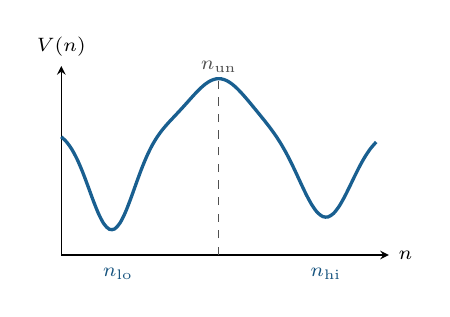
\begin{tikzpicture}[scale=0.80,>=stealth,every node/.style={font=\scriptsize}]
  \draw[->](0,0)--(5.2,0)node[right]{$n$};
  \draw[->](0,0)--(0,3.0)node[above]{$V(n)$};
  \draw[very thick,myblue!80!black,smooth]
    plot[domain=0:5,samples=60]
    (\x,{2.0-1.6*exp(-4*(\x-0.8)^2)-1.4*exp(-3*(\x-4.2)^2)+0.8*exp(-2.5*(\x-2.5)^2)});
  \node[fastblue!70!black] at (0.9,-0.3){$n_{\rm lo}$};
  \node[fastblue!70!black] at (4.2,-0.3){$n_{\rm hi}$};
  \draw[dashed,mygray,thin](2.5,0)--(2.5,2.8);
  \node[mygray,above] at (2.5,2.75){$n_{\rm un}$};
\end{tikzpicture}

\vspace{0.6em}
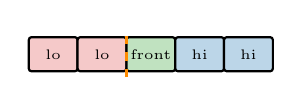
\begin{tikzpicture}[scale=0.62,every node/.style={font=\tiny}]
  \foreach \k/\col/\lbl in {
      1/slowred!25/lo,2/slowred!25/lo,
      3/activegreen!30/{front},4/myblue!30/hi,5/myblue!30/hi}{
    \draw[thick,fill=\col,rounded corners=1pt](\k-1,0)rectangle(\k,0.7);
    \node at (\k-0.5,0.35){\lbl};
  }
  \draw[very thick,intercolor,dashed](2,-0.12)--(2,0.86);
\end{tikzpicture}
\end{center}
\end{columns}

\end{frame}


% ================================================================
%  7. Schlögl 2D droplet result
% ================================================================
\begin{frame}{Result: Schl\"{o}gl critical droplet on a $60{\times}60$ grid}
\begin{center}
  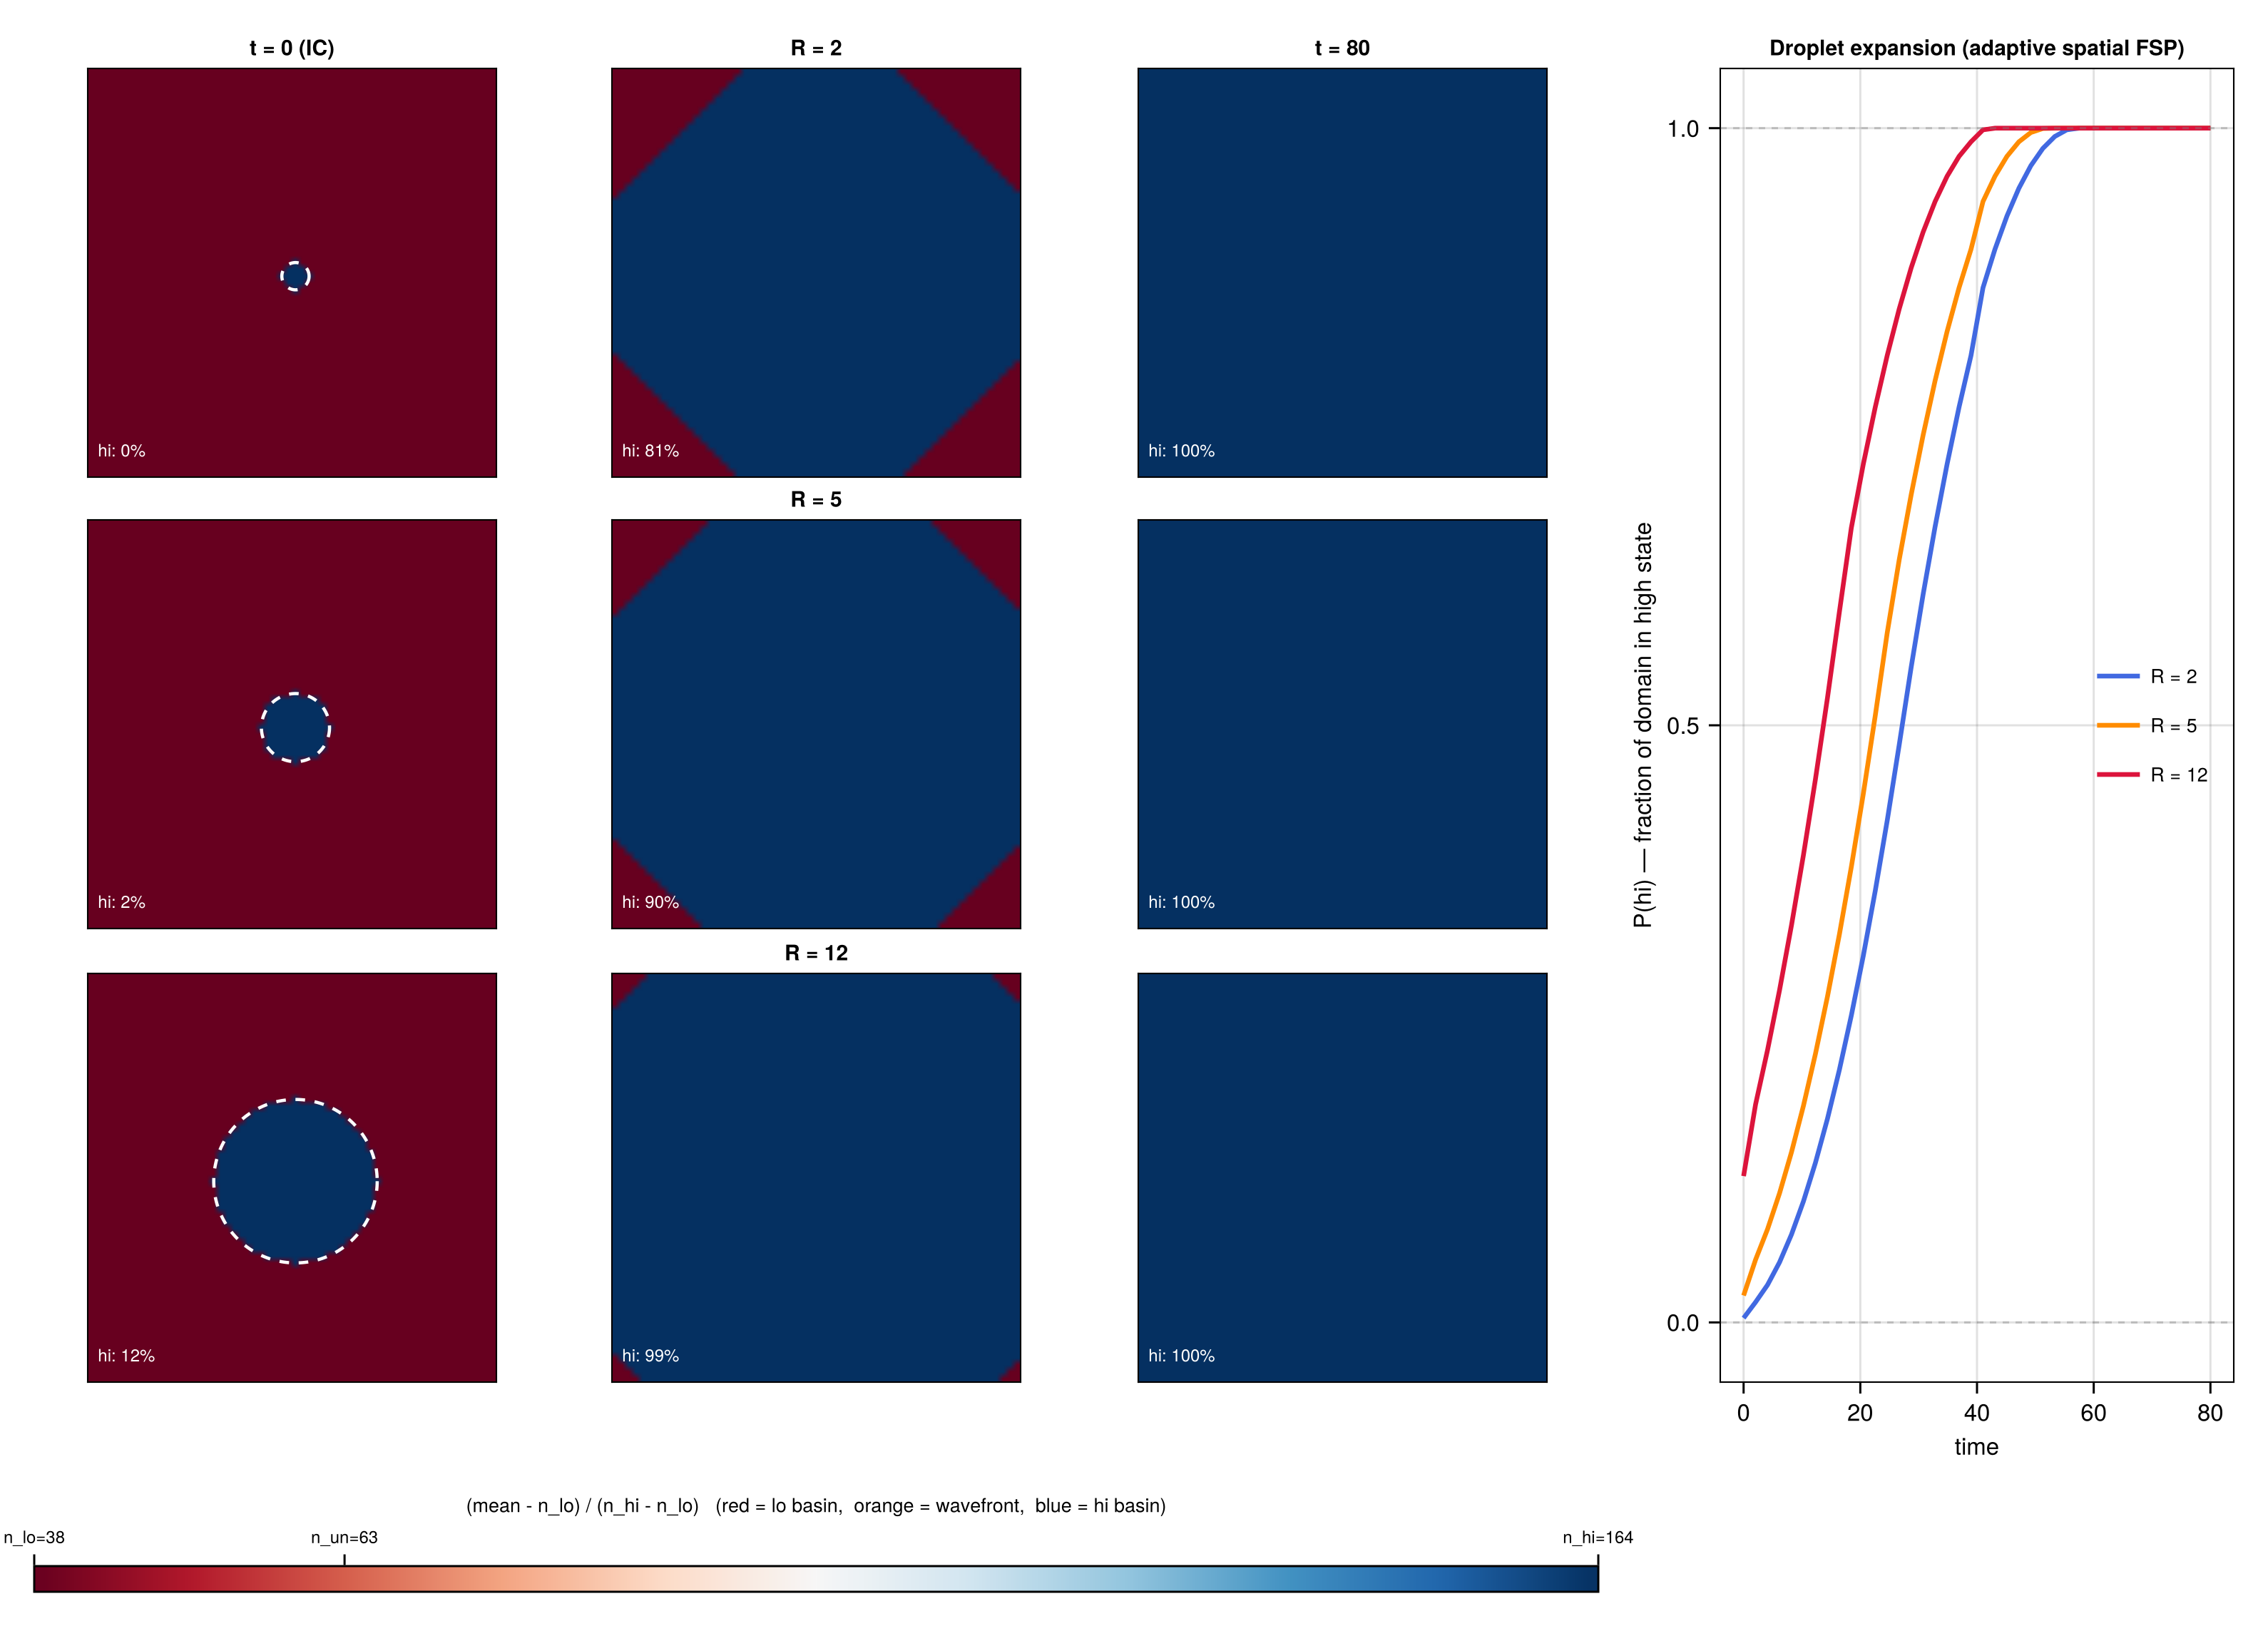
\includegraphics[width=0.90\textwidth,keepaspectratio]{fig_schlogl_2d_droplet}
\end{center}
\vspace{-0.4em}
{\footnotesize
  Schl\"{o}gl RDME, $60{\times}60$, $D{=}2.0$, $c_3{=}21$ (high state globally preferred).
  Adaptive spatial FSP. Three initial radii $R{=}2,5,12$.
  Color: $P(n > n_{\rm un})$ (red=lo, white=front, blue=hi).\\
  \textbf{Right}: fraction of voxels in high basin vs.\ time --- all radii grow.
  Bistable equil voxels are frozen at their basin ($\delta_{n_{\rm lo}}$ or $\delta_{n_{\rm hi}}$);
  per-voxel expv evolves only the thin active transition ring.
  Circular geometry is captured without anisotropy.
}
\end{frame}


% ================================================================
%  8. Correction field
% ================================================================
\begin{frame}{The correction field: L2 adds information at the front}
\begin{center}
  \includegraphics[width=0.88\textwidth,keepaspectratio]{fig_mg_correction}
\end{center}
\vspace{-0.4em}
{\footnotesize
  $200{\times}200$ BD RDME at peak wavefront ($t{=}142$, $4138$ active voxels).\\
  \textbf{Left}: $\langle n_\mathbf{k}\rangle$ heatmap --- thin active ring visible.
  \textbf{Right}: per-voxel correction $\|\Delta p_k\|_1$ applied by the L2$\to$L0 step.\\[0.2em]
  The L2 quad coarse solve updates \textbf{only at the wavefront} --- near-zero in
  the equilibrated interior.  This confirms the multigrid hierarchy is non-redundant:
  the L2 level captures collective 4-voxel dynamics that per-voxel expv cannot see.
}
\end{frame}


% ================================================================
%  9. Space-time xt diagram
% ================================================================
\begin{frame}{Space-time diagram: each level sees the wavefront differently}
\begin{center}
  \includegraphics[width=0.94\textwidth,keepaspectratio]{fig_mg_spacetime}
\end{center}
\vspace{-0.4em}
{\footnotesize
  Heatmap: radial mean $\langle n\rangle$ vs.\ radius (x) and time (y).
  White dashed: theoretical $v{\approx}1.26$.\\
  \textbf{L0} (per-voxel): sharp thin band.
  \textbf{L1} (2-voxel smooth): slightly broader front.
  \textbf{L2} (4-voxel smooth): broadest --- quads capture collective dynamics
  \emph{ahead} of the fine-level front.\\[0.2em]
  Non-redundancy across levels is why the hierarchy works:
  each level carries distinct spatial-scale information that the others cannot resolve.
}
\end{frame}


% ================================================================
%  10. Summary
% ================================================================
\begin{frame}{Summary}

  \begin{block}{1.\quad Adaptive voxel classification with Galerkin-reduced CME.}
    The full RDME ($n_{\max}^{K^2}$ states) is never assembled.
    \textbf{Equilibrated} voxels track the full distribution, evolved cheaply via a
    single-voxel Galerkin CME with effective rates from neighbour means.
    \textbf{Empty} voxels are activated organically as the wavefront advances.
  \end{block}

  \bigskip
  \begin{block}{2.\quad Spatial multigrid V-cycle at the active front.}
    Three-level hierarchy: L0 (voxels) $\to$ L1 (pairs) $\to$ L2 (quads).
    Restriction by convolution; coarse CME solve captures 4-voxel collective dynamics;
    multiplicative correction propagates L2$\to$L1$\to$L0.
    Time is split exactly: $\alpha_{\rm pre} + (1{-}2\alpha) + \alpha_{\rm post} = \Delta t$.\\[0.2em]
    \emph{${\sim}40\%$ speedup on $200{\times}200$ BD wavefront.
    Correction field confirms L2 acts only at the active front.}
  \end{block}

  \bigskip
  \begin{block}{3.\quad Model-agnostic: handles bistability natively.}
    Schl\"{o}gl equil voxels are frozen at their basin ($n_{\rm lo}$ or $n_{\rm hi}$);
    re-activated only when wavefront flux crosses $n_{\rm un}$.
    The multigrid evolves only the thin transitioning front.
    Circular droplets on $60{\times}60$ with correct P(hi) dynamics.\\[0.2em]
    \emph{No special-casing for bistability: identical algorithm, different model dispatch.}
  \end{block}

\end{frame}


\end{document}
